\graphicspath{{content/2_design/figures/}}
\section{Range sensor}
\subsection{Sensor power \& output}
The range sensor requires \SI{5}{V_{dc}} power and will draw around \SI{15}{mA}. Since the LD1117V provides a stable 5.0 V output and is capable
of providing up to 800 mA of current, the sensor will be powered directly from this regulator.

The sensor's output is a PWM wave of varying duty cycle $\tau$. Since a 16 Hz trigger will be used, the output signal
will have $f_{PWM} = \SI{16}{Hz}$. This signal's amplitude could be as high as 5 V (TTL level). The maximum output $A_{max}$ \textit{after} unity filtering,
however, will be determined by the maximum duty cycle, $t_{max}$. Since a distance of $D_{max} = \SI{1}{m}$ and $D_{min} = \SI{5}{cm}$,
Equations \ref{eqn:sensor_distanceFormula} and \ref{eqn:pwm_filtered_amplitude} can be used to calculate:
\begin{itemize}
  \item At $D_{max}$, $t_{max} \approx \SI{5.9}{ms}$, $\tau_{max} = \frac{\SI{5.9}{ms}}{1/16} \approx 9.5 \%$ and $A_{max} = (\SI{5}{V}) \cdot (9.5 \%) = \SI{475}{mV} $.
  \item At $D_{min}$, $t_{min} \approx \SI{0.29}{ms}$, $\tau_{min} = \frac{\SI{0.29}{ms}}{1/16} \approx 0.47 \%$ and $A_{min} = (\SI{5}{V}) \cdot (0.47 \%) = \SI{23}{mV} $.
\end{itemize}

\subsection{Filter selection}{\label{rangeSensor_design_filter}}

To determine the filter's order, rise time and noise requirements should be considered:
\begin{itemize}
  \item After filtering, since gain = $\frac{\SI{3}{V}}{\SI{475}{mV}} \approx \SI{7}{V/V}$, filter ripple must be under $ \frac{\SI{70}{mV}}{7} = \SI{7}{mV}$.
  \item A 10\% to 90\% rise time ($t_r$) of \SI{1.5}{s} should be adhered to.
\end{itemize}

These specifications result in the requirement that $A_{dB}$ at $f_{PWM} = 20 \log \left[ \frac{\SI{5}{V}}{\SI{7}{mV}} \right] \approx \SI{60}{dB}$.

\begin{table}[!h]
  \centering
  \renewcommand{\arraystretch}{1.2}
  \begin{tabular}{ |c|c|p{2.5cm}|p{2.5cm}|p{3.5cm}| }
    \hline
    \textbf{Filter type}  & \textbf{Design Spec.}         & \textbf{Cutoff $f_c$}     & \textbf{Rise time $t_r$}        & \textbf{Attenuation $A_{dB}$}       \\
    \hline
    \nth{1} order            & Rise Time                     & 0.233 Hz                  & 1.5 s                           & 37 dB                               \\
                             & Attenuation                   & 0.016 Hz                  & 22 s                            & 60 dB                               \\ \hline
    \nth{2} order            & Rise Time                     & 0.350 Hz                  & 1.5 s                           & 66 dB                               \\
                             & Attenuation                   & 0.505 Hz                  & 1.038 s                         & 60 dB                               \\ \hline
    \nth{3} order (cascade)  & Rise Time                     & 0.420 Hz                  & 1.5 s                           & 95 dB                               \\
                             & Attenuation                   & 1.600 Hz                  & 0.394 s                         & 60 dB                               \\ \hline
  \end{tabular}
  \caption{Filter type vs Rise Time and Attenuation using [\ref{filter_formulae}]}
  \label{tab:range_sensor_filter_comparison}
\end{table}

Referring to \ref{tab:range_sensor_filter_comparison}, the \nth{2} order provides results that will theoretically work,
but may be very sensitive to component tolerances. A \nth{3} order filter will therefore be used in this design.

\subsection{Circuit configuration}

A "two-and-a-half" stage configuration will be used. The first stage will be a \nth{2} order filter to remove PWM harmonics.
The second stage will be a gain and \nth{1} order filter stage. A Sallen-Key topology will be used for stage 1,
as in Figure \ref{fig:sallenKeyFilter}, and a non-inverting amplifier with filtering will be used for stage 2, as in Figure \ref{fig:opamp-non-inverting-filter}.

\subsection{Filter design}

A cutoff frequency of $f_c = \SI{0.6}{Hz}$ will be used, providing $t_r \approx 1.1 s$ and $A_{dB} \approx 86 dB $ for the combined \nth{3} order filter [\ref{filter_formulae}].
This results in the \nth{2} order stage transfer function $H(s) = \frac{1}{1 + 0.3751 s + 0.07036 s^2} = \frac{1}{1 + a_1 s + b_1 s^2}$. Now, component values can be chosen.
A number of formulae from \cite{filterDesign} will be used:

\begin{itemize}
  \item The idle current of this stage is very low, since both capacitors are open-circuit during DC. A maximum step input will result in a surge of current from the input through $C_2$ to ground.
        With $V_{in(max)} = \SI{5}{V}$, choose $R_1 + R_2 >> \frac{\SI{5}{V}}{\SI{250}{\micro\ampere}} = \SI{20}{\kilo\ohm}$.
  \item Since $C_1 = \frac{a_1}{2 \pi f_c (R_1 + R_2)}$ \cite{filterDesign}, choose $C_1 = \SI{220}{nF}$ so that $R_1 + R_2 = \SI{450}{\kilo\ohm}$.
  \item To meet $C_2 \geq C_1 \cdot \frac{4 \cdot b_1}{a_1 ^2} $\cite{filterDesign} $\approx 2 C_1 $, choose $C_2 = \SI{470}{nF}$.
  \item Since $C_1 \cdot C_2 = \frac{b_1}{((2 \pi f_c)^2 R_1 R_2)}$, and $R_1 + R_2 = \SI{450}{\kilo\ohm}$ solve to obtain $R_1 = \SI{170}{\kilo\ohm}$ and $R_2 = \SI{280}{\kilo\ohm}$.
        Choose $R_1 = \SI{180}{\kilo\ohm}$ and $R_2 = \SI{270}{\kilo\ohm}$ as practical values.
\end{itemize}

\begin{figure}[!htb]
  \centering
  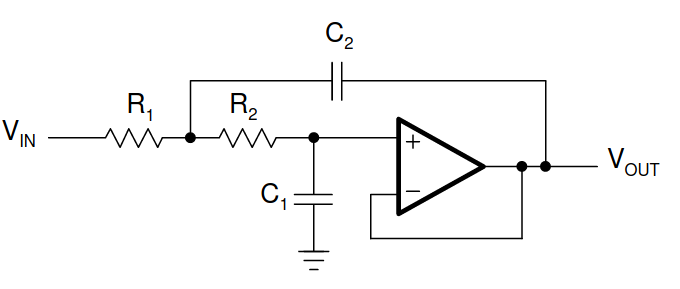
\includegraphics[width=0.4\textwidth]{rangeSensor_sallenKeyFilter}
  \caption{\nth{2} order unity-gain Sallen-Key LPF \cite{filterDesign}}
  \label{fig:sallenKeyFilter}
\end{figure}

\subsection{Amplifier design}

The amplifier circuit will 